\documentclass[12pt]{article} 
\usepackage[letterpaper, margin=0.5in]{geometry}        		
\geometry{letterpaper}
\usepackage[parfill]{parskip} 
\usepackage{framed}
\usepackage{graphicx}
\usepackage{amsmath}
\usepackage{amssymb}
\usepackage{qtree}
\usepackage{makecell}

\usepackage{lmodern}
\renewcommand*\familydefault{\sfdefault}

\usepackage{tikz}
\usetikzlibrary{matrix}

\usepackage{mathtools}
\DeclarePairedDelimiter\ceil{\lceil}{\rceil}
\DeclarePairedDelimiter\floor{\lfloor}{\rfloor}
\DeclarePairedDelimiter\abs{\lvert}{\rvert}%
\DeclarePairedDelimiter\norm{\lVert}{\rVert}%
    % \abs & \norm resizes brackets, starred version doesn't
    \makeatletter
    \let\oldabs\abs
    \def\abs{\@ifstar{\oldabs}{\oldabs*}}
    %
    \let\oldnorm\norm
    \def\norm{\@ifstar{\oldnorm}{\oldnorm*}}
    \makeatother
    
\newcommand{\addend}{\text{\textsl{\color{gray}{Addend}}}}
\newcommand{\augend}{\text{\textsl{\color{gray}{Augend}}}}
\newcommand{\sumOut}{\text{\textsl{\color{gray}{Sum}}}}

\newcommand\graytag[1]{\text{\textsl{\color{gray}{#1}}}}

    
\newcommand\tab[1][0.25cm]{\hspace*{#1}}
\newcommand\imp{\rightarrow}
\newcommand\thfr{\tab \therefore \tab}
\newcommand\sameas{\tab \equiv \tab}

\title{CSC263 - Week 2, Lecture 2}
\author{Cristyn Howard}
\date{Wednesday, January 17, 2018}

\begin{document}
\maketitle


\begin{center}
\begin{tabular}{|c|c|c|}
\hline
ADT & Data Structure & Operations \\
\hline
Mergeable Priority Queues & Binomial Heap & insert, min, extract-min, merge \\
\hline
\end{tabular}
\end{center}
\vspace{0.4cm}

MERGE:
	\begin{itemize}
	\item Merging two binary forests is directly analogous to adding two binary numbers.
	\item Any time both of the forests being added each have an $S_k$ tree of the same size, they merge to form a new $S_{k+1}$ tree. 
	\item This is the equivalent of adding two 1's in the same digit of two binary numbers, and carrying the 1 to the next column.
	\end{itemize}

\begin{center}
\begin{tabular}{c|c}

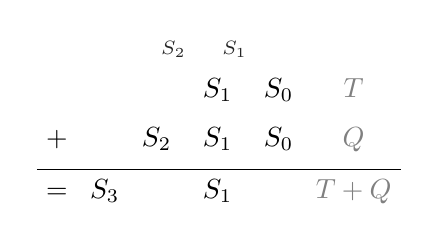
\begin{tikzpicture}[
	row 1/.style={font=\textsl,font=\scriptsize,black!85, anchor=west,inner sep=1.5pt},
	every node/.style={column sep=.5mm,row sep=1mm}]
	\matrix (m) [matrix of math nodes,nodes in empty cells] 
    {
        &   & S_2  & S_1  &   &               \\
        &   &   &  S_1 & S_0 &[10mm]     \graytag{$T$} \\
    +   &   & S_2 & S_1 & S_0 &           \graytag{$Q$} \\ 
    \hline
    =   & S_3 &   & S_1 &   &           \graytag{$T+Q$} \\                                                  
    };
 	\draw[-,color=black,semithick];
 \end{tikzpicture} 
 
 & 
 
 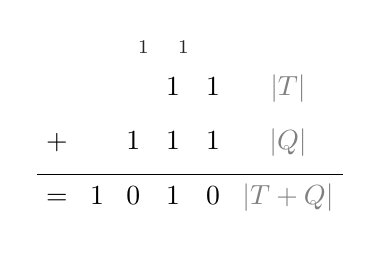
\begin{tikzpicture}[
	row 1/.style={font=\textsl,font=\scriptsize,black!85, anchor=west,inner sep=1.5pt},
	every node/.style={column sep=.5mm,row sep=1mm}]
	\matrix (m) [matrix of math nodes,nodes in empty cells] 
    {
        &   & 1 & 1 &   &               \\
        &   &   &  1 & 1 &[10mm]     \graytag{$\abs{T}$} \\
    +   &   & 1 & 1 & 1 &           \graytag{$\abs{Q}$} \\ 
    \hline
    =   & 1 & 0 & 1 & 0 &           \graytag{$\abs{T+Q}$} \\                                                  
    };
 	\draw[-,color=black,semithick];
 \end{tikzpicture} 
 \\
 
\end{tabular}
\end{center}

	\begin{itemize}
	\item Every time a tree is "carried" to the next column, it indic
	\end{itemize}






\end{document}